\documentclass[a4paper,UTF8]{article}
\usepackage{ctex}
\usepackage[margin=1.25in]{geometry}
\usepackage{color}
\usepackage{graphicx}
\usepackage{amssymb}
\usepackage{amsmath}
\usepackage{amsthm}
\usepackage{enumerate}
\usepackage{bm}
\usepackage{hyperref}
\numberwithin{equation}{section}
%\usepackage[thmmarks, amsmath, thref]{ntheorem}
\theoremstyle{definition}
\newtheorem*{solution}{Solution}
\newtheorem*{prove}{Proof}
\usepackage{multirow}

%--

%--
\begin{document}
\title{机器学习导论\\
习题四}
\author{141220120, 徐世坚, xsj13260906215@gmail.com}
\maketitle
\section{\textbf{[20pts]} Reading Materials on CNN}
卷积神经网络(Convolution Neural Network,简称CNN)是一类具有特殊结构的神经网络,在深度学习的发展中具有里程碑式的意义。其中,Hinton于2012年提出的\href{https://en.wikipedia.org/wiki/AlexNet}{AlexNet}可以说是深度神经网络在计算机视觉问题上一次重大的突破。

关于AlexNet的具体技术细节总结在经典文章\href{https://papers.nips.cc/paper/4824-imagenet-classification-with-deep-convolutional-neural-networks}{“ImageNet Classification with Deep Convolutional Neural Networks”}, by Alex Krizhevsky, Ilya Sutskever and Geoffrey E. Hinton in NIPS'12,目前已逾万次引用。在这篇文章中,它提出使用ReLU作为激活函数,并创新性地使用GPU对运算进行加速。请仔细阅读该论文,并回答下列问题(请用1-2句话简要回答每个小问题,中英文均可)。

\begin{enumerate}[(a)]
\item \textbf{[5pts]} Describe your understanding of how ReLU helps its success? And, how do the GPUs help out?
\item \textbf{[5pts]} Using the average of predictions from several networks help reduce the error rates. Why?
\item \textbf{[5pts]} Where is the dropout technique applied? How does it help? And what is the cost of using dropout?
\item \textbf{[5pts]} How many parameters are there in AlexNet? Why the dataset size(1.2 million) is important for the success of AlexNet?
\end{enumerate}

关于CNN,推荐阅读一份非常优秀的学习材料,由南京大学计算机系吴建鑫教授\footnote{吴建鑫教授主页链接为\url{cs.nju.edu.cn/wujx}}所编写的讲义Introduction to Convolutional Neural Networks\footnote{由此链接可访问讲义\url{https://cs.nju.edu.cn/wujx/paper/CNN.pdf}},本题目为此讲义的Exercise-5,已获得吴建鑫老师授权使用。
\begin{solution}
此处用于写解答(中英文均可)\\
(a)The ReLU helps their model learns several times faster than equivalents with saturating neurons (the sigmoid function or tanh function) on such a large dataset.\\
The parallelization scheme with two GPUs and the trick that the GPUs communicate only in certain layers help the model take less time to train and reduce the error rate.\\
(b)Because this can reduce the effect of overfitting and make the model more robust.\\
(c)Dropout is used in the first two fully-connected layers. \\
It reduces complex co-adaptations of neurons and forces the model to learn more robust features that are useful in conjunction with many different random subsets of the other neurons, which helps reduce the effect of overfitting. \\
The cost is that dropout roughly doubles the number of iterations required to converge.\\
(d)There are 60 million parameters. Because there are too many parameters, if the dataset is not large enough, then the model is very likely to have considerable overfitting.\\
~\\
\end{solution}

\section{[20pts] Kernel Functions}
\begin{enumerate}[(1)]
\item 试通过定义证明以下函数都是一个合法的核函数:
	\begin{enumerate}[(i)]
	\item \textbf{[5pts]} 多项式核: $\kappa(\mathbf{x}_i,\mathbf{x}_j) = (\mathbf{x}_i^\mathrm{T}\mathbf{x}_j)^d$;
	\item \textbf{[10pts]} 高斯核:$\kappa(\mathbf{x}_i,\mathbf{x}_j) = \exp(-\frac{\lVert \mathbf{x}_i - \mathbf{x}_j \rVert^2}{2\sigma^2})$, 其中$\sigma > 0$.
	\end{enumerate}
\item \textbf{[5pts]} 试证明$\kappa(\mathbf{x}_i,\mathbf{x}_j)=\frac{1}{1+e^{-\mathbf{x}_i^T\mathbf{x}_j}}$不是合法的核函数。
\end{enumerate}
\begin{prove}
此处用于写证明(中英文均可)\\
(1)(i)According to the definition, a function is a kernel function if there exist a mapping $\Phi$ such that the function can be presented as $ k(\mathbf x, \mathbf y) =\Phi(\mathbf x)^T \Phi(\mathbf y)$.\\
$\kappa(\mathbf{x}_i,\mathbf{x}_j) = (\mathbf{x}_i^\mathrm{T}\mathbf{x}_j)^d$\\
$= (\sum_{k=1}^n x_{ik}x_{jk})^d$\\
$= \sum \frac{d!}{d_1!d_2!...d_n!}(x_{i_1}x_{j_1})^{d_1} (x_{i_2}x_{j_2})^{d_2} ... (x_{i_n}x_{j_n})^{d_n}$\\
$= \sum \frac{d!}{d_1!d_2!...d_n!}(x_{i_1}^{d_1} x_{i_2}^{d_2} ... x_{i_n}^{d_n})(x_{j_1}^{d_1} x_{j_2}^{d_2} ... x_{j_n}^{d_n})$\\
$= \sum (\sqrt{\frac{d!}{d_1!d_2!...d_n!}} x_{i_1}^{d_1} x_{i_2}^{d_2} ... x_{i_n}^{d_n})(\sqrt{\frac{d!}{d_1!d_2!...d_n!}} x_{j_1}^{d_1} x_{j_2}^{d_2} ... x_{j_n}^{d_n})$\\
$= \Phi(\mathbf x_i)^T \Phi(\mathbf x_j)$\\
in which, $\sum_i^n d_i = d$, and $0 \leq d_i \leq d$.\\
$\therefore (\mathbf{x}_i^\mathrm{T}\mathbf{x}_j)^d$   is a valid kernel function.\\
(ii)$\kappa(\mathbf{x}_i,\mathbf{x}_j) = \exp(-\frac{\lVert \mathbf{x}_i - \mathbf{x}_j \rVert^2}{2\sigma^2})$\\
$= \exp(-\frac{\lVert \mathbf{x}_i \rVert^2}{2\sigma^2})\exp(-\frac{\lVert \mathbf{x}_j \rVert^2}{2\sigma^2})\exp(\frac{\mathbf{x}_i^T \mathbf{x}_j}{\sigma^2})$\\
$= \exp(-\frac{\lVert \mathbf{x}_i \rVert^2}{2\sigma^2})\exp(-\frac{\lVert \mathbf{x}_j \rVert^2}{2\sigma^2})  \sum_{k=0}^{\infty}\frac{1}{k!}(\frac{\mathbf{x}_i^T\mathbf{x}_j}{\sigma^2})^k$\\
$= \sum_{k=0}^{\infty} \exp(-\frac{\lVert \mathbf{x}_i \rVert^2}{2\sigma^2})\exp(-\frac{\lVert \mathbf{x}_j \rVert^2}{2\sigma^2}) \frac{1}{k!}(\frac{\mathbf{x}_i^T\mathbf{x}_j}{\sigma^2})^k$\\
$= \sum_{k=0}^{\infty} (\exp(-\frac{\lVert \mathbf{x}_i \rVert^2}{2\sigma^2 k})  \exp(-\frac{\lVert \mathbf{x}_j \rVert^2}{2\sigma^2 k })  \frac{1}{(k!)^{1/k}} \frac{\mathbf{x}_i^T\mathbf{x}_j}{\sigma^2})^k $\\
$= \sum_{k=0}^{\infty}  ( ( \exp(-\frac{\lVert \mathbf{x}_i \rVert^2}{2\sigma^2 k}) \frac{1}{(k!)^{1/2k}} \frac{1}{\sigma} \mathbf{x}_i )^T ( \exp(-\frac{\lVert \mathbf{x}_j \rVert^2}{2\sigma^2 k }) \frac{1}{(k!)^{1/2k}} \frac{1}{\sigma} \mathbf{x}_j) )^k $\\
$= \sum_{k=0}^{\infty}  \sum  (\sqrt{\frac{k!}{k_1!k_2!...k_n!}} \exp(-\frac{\lVert \mathbf{x}_i \rVert^2}{2\sigma^2} \frac{1}{(k!)^{1/2}} \frac{1}{\sigma^k} x_{i_1}^{k_1} x_{i_2}^{k_2} ... x_{i_n}^{k_n} ) ( \sqrt{\frac{k!}{k_1!k_2!...k_n!}} \exp(-\frac{\lVert \mathbf{x}_j \rVert^2}{2\sigma^2} \frac{1}{(k!)^{1/2}} \frac{1}{\sigma^k} x_{j_1}^{k_1} x_{j_2}^{k_2} ... x_{j_n}^{k_n})$\\
$= \Phi(\mathbf x_i)^T \Phi(\mathbf x_j)$\\
in which, $\sum_i^n k_i = k$, and $0 \leq k_i \leq k$.\\
$\therefore \exp(-\frac{\lVert \mathbf{x}_i - \mathbf{x}_j \rVert^2}{2\sigma^2})$   is a valid kernel function.\\
(2)Let $D={\mathbf{x}_1, \mathbf{x}_2}$\\
$\mathbf{x}_1=[1, 1]^T, \mathbf{x}_2=[2, 2]^T$\\
Then, the kernel matrix for this D is:\\
$$\left[
 \begin{matrix}
   \frac{1}{1+e^{-2}} & \frac{1}{1+e^{-4}}  \\
   \frac{1}{1+e^{-4}} & \frac{1}{1+e^{-8}}
  \end{matrix}
  \right]$$\\
$\because det= -0.08384 < 0$\\
$\therefore$ the kernel matrix is not PSD, so this function is not a valid kernel function.\\
\qed
\end{prove}

\section{[25pts] SVM with Weighted Penalty}
考虑标准的SVM优化问题如下(即课本公式(6.35)),
\begin{equation}
\label{eq-svm}
\begin{split}
\min_{\mathbf{w},b,\xi_i}& \quad \frac{1}{2} \lVert \mathbf{w} \rVert^2 + C\sum_{i=1}^m\xi_i\\
\text{s.t.}&  \quad y_i(\mathbf{w}^\mathrm{T}\mathbf{x}_i + b)\geq 1-\xi_i\\
& \quad \xi_i \geq 0, i = 1,2,\cdots,m.
\end{split}
\end{equation}

注意到,在\eqref{eq-svm}中,对于正例和负例,其在目标函数中分类错误的“惩罚”是相同的。在实际场景中,很多时候正例和负例错分的“惩罚”代价是不同的,比如考虑癌症诊断,将一个确实患有癌症的人误分类为健康人,以及将健康人误分类为患有癌症,产生的错误影响以及代价不应该认为是等同的。

现在,我们希望对负例分类错误的样本(即false positive)施加$k>0$倍于正例中被分错的样本的“惩罚”。对于此类场景下,

(1) \textbf{[10pts]} 请给出相应的SVM优化问题;

(2) \textbf{[15pts]} 请给出相应的对偶问题,要求详细的推导步骤,尤其是如KKT条件等。
\begin{solution}
此处用于写解答(中英文均可)\\
(1)\begin{equation}
\begin{split}
\min_{\mathbf{w},b,\xi_i}& \quad \frac{1}{2} \lVert \mathbf{w} \rVert^2 + C_1\sum_{i\in S_+} \xi_i + C_2\sum_{i\in S_-}\xi_i\\
\text{s.t.}&  \quad y_i(\mathbf{w}^\mathrm{T}\mathbf{x}_i + b)\geq 1-\xi_i\\
& \quad \xi_i \geq 0, i = 1,2,\cdots,m\\
& \quad C_2 = k C_1 \\
& \quad k > 0.
\end{split}
\end{equation}
(2)\begin{equation}
\begin{split}
L(\mathbf{\omega},b,\mathbf{\alpha},\mathbf{\xi},\mathbf{\mu})= & \frac{1}{2} \lVert \mathbf{w} \rVert^2 + C_1\sum_{i\in S_+} \xi_i + C_2\sum_{i\in S_-}\xi_i\\
& + \sum_{i=1}^m \alpha_i(1-\xi_i-y_i(\mathbf{\omega}^T\mathbf{x}_i+b))-\sum_{i=1}^{m}\mu_i\xi_i,\\
\end{split}
\end{equation}
in which, $\alpha_i \geq 0, \mu_i\geq 0 $ are Lagrange multipliers, and $C_2 = kC_1$.\\
Let the partial derivative of $L(\mathbf{\omega},b,\mathbf{\alpha},\mathbf{\xi},\mathbf{\mu})$ with respect to $\mathbf{\omega}, b, \xi_i$ be zero\\
\begin{equation}
\begin{split}
& \mathbf{\omega} = \sum_{i=1}^m \alpha_i y_i \mathbf{x}_i \\
& 0 = \sum_{i=1}^m \alpha_i y_i\\
& C_1 = \alpha_i + \mu_i, i\in S_+\\
& C_2 = \alpha_i + \mu_i, i\in S_-\\
\end{split}
\end{equation}
put them into equation (3.3), we get\\
\begin{equation}
\begin{split}
\max_\mathbf{\alpha}& \quad \sum_{i=1}^m \alpha_i - \frac{1}{2}\sum_{i=1}^m\sum_{j=1}^{m}\alpha_i\alpha_j y_i y_j \mathbf{x}_i^T\mathbf{x}_j\\
\text{s.t.}&  \quad \sum_{i=1}^m\alpha_i y_i = 0\\
& \quad 0 \leq \alpha_i \leq C_1, i \in S_+\\
& \quad 0 \leq \alpha_i \leq C_2, i \in S_-\\
\end{split}
\end{equation}
The KKT condition is\\
\begin{equation}
\begin{split}
& \alpha_i \geq 0, \mu_i \geq 0, \\
& y_i f(\mathbf{x}_i) - 1 + \xi_i \geq 0,\\
& \alpha_i(y_i f(\mathbf{x}_i) -1 + \xi_i) = 0,\\
& \xi_i \geq 0, \mu_i\xi_i=0.\\
\end{split}
\end{equation}

\end{solution}

\section{[35pts] SVM in Practice - LIBSVM} 
支持向量机(Support Vector Machine,简称SVM)是在工程和科研都非常常用的分类学习算法。有非常成熟的软件包实现了不同形式SVM的高效求解,这里比较著名且常用的如LIBSVM\footnote{LIBSVM主页课参见链接:\url{https://www.csie.ntu.edu.tw/~cjlin/libsvm/}}。

(1) \textbf{[20pts]} 调用库进行SVM的训练,但是用你自己编写的预测函数作出预测。

(2) \textbf{[10pts]} 借助我们提供的可视化代码,简要了解绘图工具的使用,通过可视化增进对SVM各项参数的理解。详细编程题指南请参见链接:\url{http://lamda.nju.edu.cn/ml2017/PS4/ML4_programming.html}. 

(3) \textbf{[5pts]} 在完成上述实践任务之后,你对SVM及核函数技巧有什么新的认识吗?请简要谈谈。

\begin{solution}
此处用于写解答(中英文均可)\\
(1)见附件\\
(2)\\
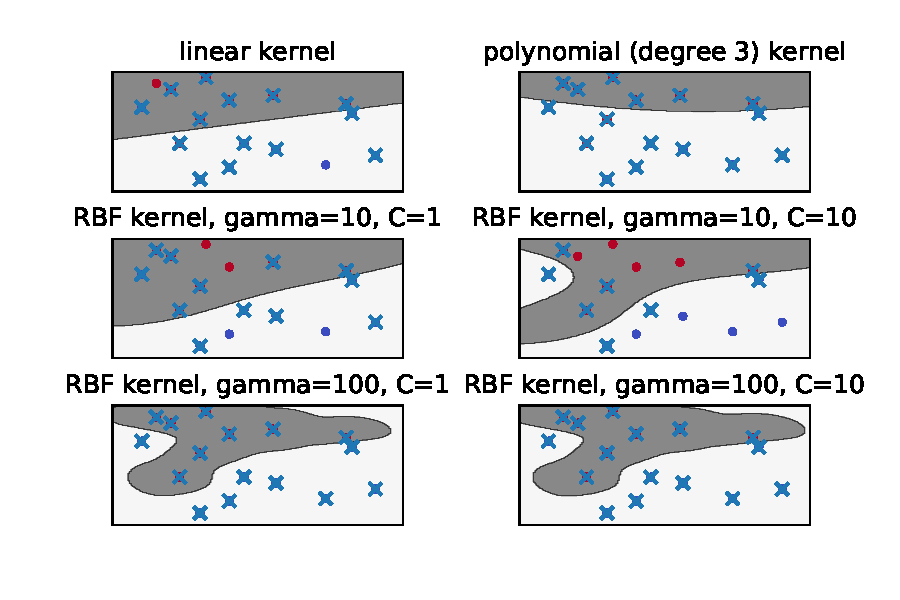
\includegraphics[height=10cm]{figure.pdf}\\
(3)学会常用的软件包工具可以大大方便SVM的实现,以及可视化工作非常有趣但也很繁琐。对于不同的核函数以及不同的参数设置,最终的超平面和支持向量都会有很大的不同。
\end{solution}


\end{document}